\externaldocument{clendshape_classification}

\chapter{Audio Driven Blendshape GAN}
This chapter shall discuss the use of GANs for audio driven facial animation.
Unlike previous generative models which solve a regression problem to correctly match an audio input to a sequence parameters which describe facial motion, GANs also include an noise input resulting in variations in the output from the same conditional input.
The model outputs will then be assessed on the classification models discussed in Chapter \ref{chap:classification}.

\section{Problem Definition}
Currently, there is a lack of 3D temporal datasets which sync speech audio with corresponding facial motion with the purpose of training a model for VSR.
Such datasets are difficult to capture directly due to the equipment and time required.
Similar datasets exist which have enabled for the creation of audio driven models but these datasets are limited in size and variation and have led to models which are specific to subjects either though direct subject specific training data as with the model by Karras et al. \cite{Karras2017a} or through character encoding, as is the case with the VOCA model \cite{Cudeiro2019}.
Through the use of these models, a synthetic dataset of 3D temporal facial motion was generated as described in Section \ref{sec:dataset_gen}.
This data however is subject to all biases and restrictions the VOCA model is subject to.
An appropriate dataset would contain a small vocabulary, similar to the LRW dataset of 500 words, all spoken by multiple subjects to capture different speaking styles for the same words captured from `\textit{in the wild}' scenarios.

An appropriate dataset would:
\begin{itemize}
    \item A small vocabulary of a similar size to the LRW dataset.
    \item Multiple subjects speaking the same vocabulary to capture different speaking styles for the same words.
    \item ``\textit{In the wild}'' audio conditions.
\end{itemize}

As a means to increase the variation in speaking style in existing audio drive generative models such as VOCA, a GAN model is to be trained on the data generated by the VOCA model and the original LRW audio from which the VOCA generated dataset was driven from.
The resulting generative model should be able to replicate the results of the VOCA model, but with increased variation in speaking styles due to the noise input component.

\section{Model Inputs}
The generative model is to be driven from an audio input of audio samples from the LRW dataset which were used as inputs to the VOCA model to generate the dataset of blendshape parameters.
Audio data in the time domain has a high number of samples per second to allow all frequencies observable by human hearing to be captured.
Human hearing can commonly hear up to 20kHz, which results in a sample rate of at least 40kHz to meet the Nyquist sampling rate, which states that the sample rate must be at least twice the desired maximum observable frequency to accurately represent the signal at this frequency.
40,000 samples for a single second is however, is a large number of samples and an inefficient data representation.
Commonly audio data is converted to the frequency domain which allows for a far more efficient means of data representation. 

\subsection{Mel-frequency Cepstral Coefficients}
Common implementations of machine learning models which use audio as in input, focused on speech, have used Mel-frequency cepstral coefficients (MFCCs) to represent audio.
\textcolor{red}{TODO add references to paper examples.}
MFCCs were inspired by human anatomy and speech, invented by Davis and Mermelstein in 1980 \cite{Davis1980}.
Human speech is naturally filtered by the shape of the shape of the mouth and vocal tract.
This envelope can be well represented by the short time power spectrum.
A large amount of information is contained within an audio sample in the time domain, much of which does not contain meaningful information.
By filtering the audio sample in the frequency domain to this envelope, information useful to speech detection is maintained while other information is discarded.

Firstly the assumption that over a short time frame, the audio signal does not statistically vary greatly.
This assumption allows the signal to be split into short frames which can be processed separately.
An example of the audio frames is show in Figure \ref{fig:mfcc_audio_frames}.

\begin{figure}[h!]
    \centering
        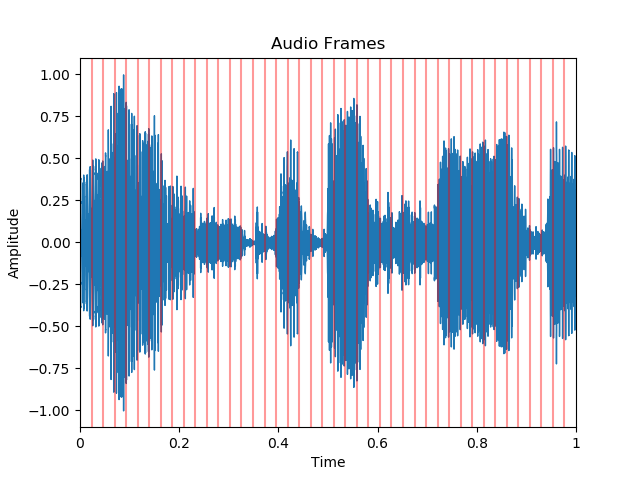
\includegraphics[width=0.7\textwidth]{figures/mfcc/audio_frames.png}
    \caption{Audio Sample Frames}
\end{figure} \label{fig:mfcc_audio_frames}

For each frame the power spectrum is calculated using the periodogram estimation.  
The incentive behind calculating the power spectrum is derived from human anatomy, specifically from the cochlea.
The cochlea is a bone which resides within the ear and different parts of the bone vibrate depending on the frequency of the incoming audio signal.
The periodogram estimation of the power spectrum performs a similar operation by identifying which frequencies are present within an audio signal.
This representation still retains information which is not useful for speech recognition, for example the cochlea cannot distinguish between closely spaced frequency values, this is more apparent at higher frequencies.
The power spectrum for a single audio frame is shown in Figure \ref{fig:mfcc_power_spec}.
For this reason a series of Mel filterbanks are applied to the power spectrum and the resulting bin for each filter is summed, this gives an approximation of the energy present in each frequency region.
The Mel filterbanks are visualised in Figure \ref{fig:mfcc_mel_filterbanks}, for ease of visualisation, only 8 filterbanks are shown in these visualisations.
The log of each summation is then taken as humans do not perceive loudness on a linear scale, so the log compression matches the features more closely to what humans hear, shown in Figure \ref{fig:mfcc_log_sum}.

\begin{figure}[h!]
    \centering
    \begin{subfigure}[b]{0.49\textwidth}
        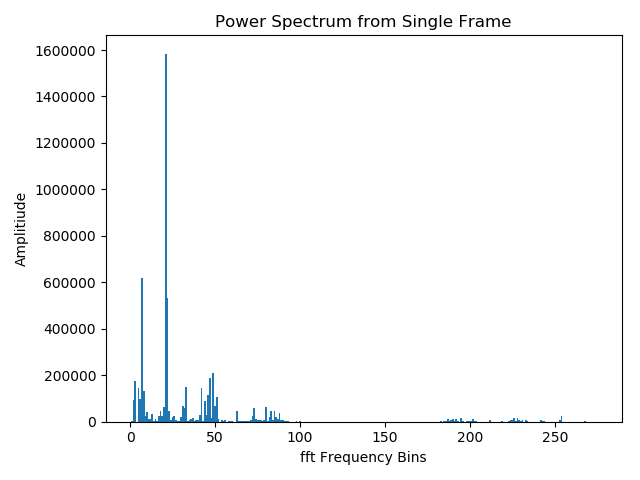
\includegraphics[width=\textwidth]{figures/mfcc/frame_power_spectrum.png}
        \caption{Audio Frame Power Spectrum}\label{fig:mfcc_power_spec}
    \end{subfigure}
    \begin{subfigure}[b]{0.49\textwidth}
        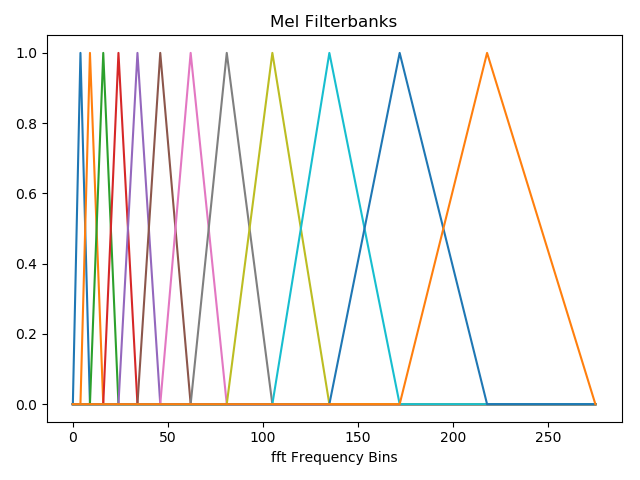
\includegraphics[width=\textwidth]{figures/mfcc/filterbanks.png}
        \caption{Mel Filterbanks}\label{fig:mfcc_mel_filterbanks}
    \end{subfigure}
    \caption{Mel Filterbank Processing}\label{fig:mfcc_filterbank_processing}
\end{figure}

Lastly, the Discrete Cosine Transformation is applied to the each filterbank energy, this is performed to decorrelate the filterbanks are they are highly correlated due to the overlap in the Mel filters, the resulting representation is shown in Figure \ref{fig:mfcc_dct}.
This represents the MFCC values for a single audio frame for 8 Mel filterbanks.

\begin{figure}[h!]
    \centering
    \begin{subfigure}[b]{0.49\textwidth}
        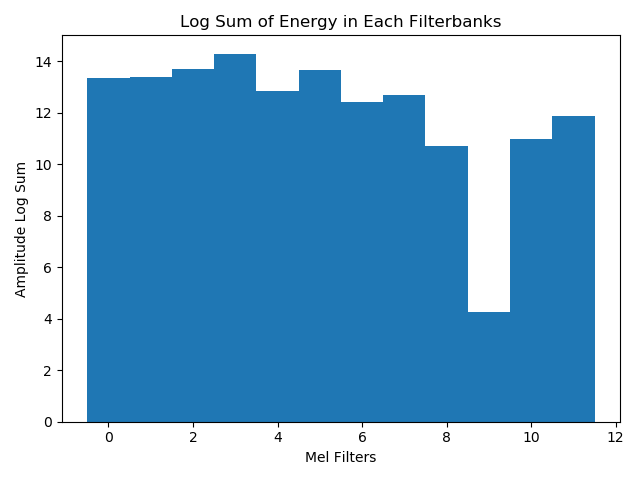
\includegraphics[width=\textwidth]{figures/mfcc/filterbank_log_sum.png}
        \caption{Log Sum}\label{fig:mfcc_log_sum}
    \end{subfigure}
    \begin{subfigure}[b]{0.49\textwidth}
        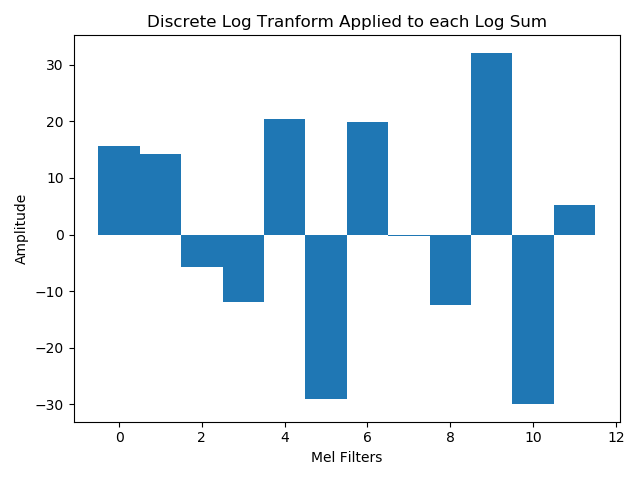
\includegraphics[width=\textwidth]{figures/mfcc/dct_applied.png}
        \caption{Discrete Cosine Transformation}\label{fig:mfcc_dct}
    \end{subfigure}
    \caption{Discrete Cosine Transformation Processing}\label{fig:mfcc_filterbank_processing}
\end{figure}

The model inputs use a total of 50 filterbanks over the span of one second audio clips.
This results in an model input MFCC $\mat{x} \in \mathbb{R}^{43 \times 50}$, visualised in Figure \ref{fig:mfcc_model_input}.

\begin{figure}[h!]
    \centering
    \begin{subfigure}[b]{0.49\textwidth}
        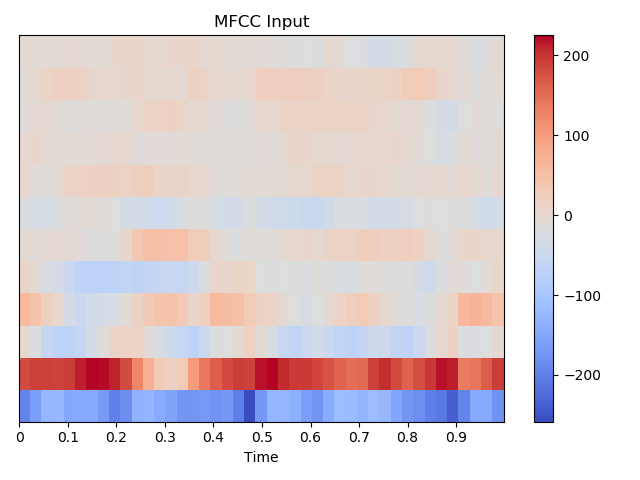
\includegraphics[width=\textwidth]{figures/mfcc/mfcc_input.png}
        \caption{MFCC Model Input}\label{fig:mfcc_input}
    \end{subfigure}
    \begin{subfigure}[b]{0.49\textwidth}
        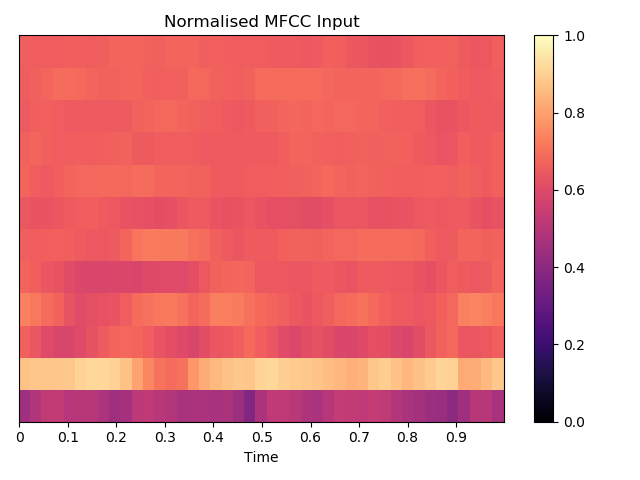
\includegraphics[width=\textwidth]{figures/mfcc/norm_mfcc_input.png}
        \caption{Normalised MFCC Model Input}\label{fig:mfcc_norm_input}
    \end{subfigure}
    \caption{MFCC Model Input}\label{fig:mfcc_model_input}
\end{figure}

\subsection{Blendshape Inputs}
The Generator aims to produce realistic blendshape parameters for the input audio signal, thus the input to the Critic must be the true blendshape parameter values and the `fake' generated blendshape parameters.
These values are the same as were input to the Blendshape Classification models discussed in Section \ref{sec:classification_inputs}: $\mat{y} \in \mathbb{R}^{43 \times 4}$.
The reader is directed to this section for further details.

\section{Data Preprocessing}
Data is normalised as before.

No need for validation set, just test set, so data training and validation set are merged.

\section{Assessment of Model Performance}

Outputs are difficult to assess as they are subjective and don't have an obvious means to quantify the quality of the results.

Generated results can be assessed by classification models discussed previously.

Variance in label outputs can be measured to see if the model has learnt new ways of saying something.
Probably only valid for labels which have been correctly labelled by (both?) classifiers.

Could conduct subjective evaluation, but this remains limited to performance of VOCA model, as are all results...

\section{Model Architecture}
Describe model arch for both critic and gen

\section{Results}

\section{Discussion}